% Options for packages loaded elsewhere
% Options for packages loaded elsewhere
\PassOptionsToPackage{unicode}{hyperref}
\PassOptionsToPackage{hyphens}{url}
\PassOptionsToPackage{dvipsnames,svgnames,x11names}{xcolor}
%
\documentclass[
  letterpaper,
  DIV=11,
  numbers=noendperiod]{scrartcl}
\usepackage{xcolor}
\usepackage{amsmath,amssymb}
\setcounter{secnumdepth}{-\maxdimen} % remove section numbering
\usepackage{iftex}
\ifPDFTeX
  \usepackage[T1]{fontenc}
  \usepackage[utf8]{inputenc}
  \usepackage{textcomp} % provide euro and other symbols
\else % if luatex or xetex
  \usepackage{unicode-math} % this also loads fontspec
  \defaultfontfeatures{Scale=MatchLowercase}
  \defaultfontfeatures[\rmfamily]{Ligatures=TeX,Scale=1}
\fi
\usepackage{lmodern}
\ifPDFTeX\else
  % xetex/luatex font selection
\fi
% Use upquote if available, for straight quotes in verbatim environments
\IfFileExists{upquote.sty}{\usepackage{upquote}}{}
\IfFileExists{microtype.sty}{% use microtype if available
  \usepackage[]{microtype}
  \UseMicrotypeSet[protrusion]{basicmath} % disable protrusion for tt fonts
}{}
\makeatletter
\@ifundefined{KOMAClassName}{% if non-KOMA class
  \IfFileExists{parskip.sty}{%
    \usepackage{parskip}
  }{% else
    \setlength{\parindent}{0pt}
    \setlength{\parskip}{6pt plus 2pt minus 1pt}}
}{% if KOMA class
  \KOMAoptions{parskip=half}}
\makeatother
% Make \paragraph and \subparagraph free-standing
\makeatletter
\ifx\paragraph\undefined\else
  \let\oldparagraph\paragraph
  \renewcommand{\paragraph}{
    \@ifstar
      \xxxParagraphStar
      \xxxParagraphNoStar
  }
  \newcommand{\xxxParagraphStar}[1]{\oldparagraph*{#1}\mbox{}}
  \newcommand{\xxxParagraphNoStar}[1]{\oldparagraph{#1}\mbox{}}
\fi
\ifx\subparagraph\undefined\else
  \let\oldsubparagraph\subparagraph
  \renewcommand{\subparagraph}{
    \@ifstar
      \xxxSubParagraphStar
      \xxxSubParagraphNoStar
  }
  \newcommand{\xxxSubParagraphStar}[1]{\oldsubparagraph*{#1}\mbox{}}
  \newcommand{\xxxSubParagraphNoStar}[1]{\oldsubparagraph{#1}\mbox{}}
\fi
\makeatother


\usepackage{longtable,booktabs,array}
\usepackage{calc} % for calculating minipage widths
% Correct order of tables after \paragraph or \subparagraph
\usepackage{etoolbox}
\makeatletter
\patchcmd\longtable{\par}{\if@noskipsec\mbox{}\fi\par}{}{}
\makeatother
% Allow footnotes in longtable head/foot
\IfFileExists{footnotehyper.sty}{\usepackage{footnotehyper}}{\usepackage{footnote}}
\makesavenoteenv{longtable}
\usepackage{graphicx}
\makeatletter
\newsavebox\pandoc@box
\newcommand*\pandocbounded[1]{% scales image to fit in text height/width
  \sbox\pandoc@box{#1}%
  \Gscale@div\@tempa{\textheight}{\dimexpr\ht\pandoc@box+\dp\pandoc@box\relax}%
  \Gscale@div\@tempb{\linewidth}{\wd\pandoc@box}%
  \ifdim\@tempb\p@<\@tempa\p@\let\@tempa\@tempb\fi% select the smaller of both
  \ifdim\@tempa\p@<\p@\scalebox{\@tempa}{\usebox\pandoc@box}%
  \else\usebox{\pandoc@box}%
  \fi%
}
% Set default figure placement to htbp
\def\fps@figure{htbp}
\makeatother





\setlength{\emergencystretch}{3em} % prevent overfull lines

\providecommand{\tightlist}{%
  \setlength{\itemsep}{0pt}\setlength{\parskip}{0pt}}



 


\KOMAoption{captions}{tableheading,figureheading}
\makeatletter
\@ifpackageloaded{caption}{}{\usepackage{caption}}
\AtBeginDocument{%
\ifdefined\contentsname
  \renewcommand*\contentsname{Table of contents}
\else
  \newcommand\contentsname{Table of contents}
\fi
\ifdefined\listfigurename
  \renewcommand*\listfigurename{List of Figures}
\else
  \newcommand\listfigurename{List of Figures}
\fi
\ifdefined\listtablename
  \renewcommand*\listtablename{List of Tables}
\else
  \newcommand\listtablename{List of Tables}
\fi
\ifdefined\figurename
  \renewcommand*\figurename{Figure}
\else
  \newcommand\figurename{Figure}
\fi
\ifdefined\tablename
  \renewcommand*\tablename{Table}
\else
  \newcommand\tablename{Table}
\fi
}
\@ifpackageloaded{float}{}{\usepackage{float}}
\floatstyle{ruled}
\@ifundefined{c@chapter}{\newfloat{codelisting}{h}{lop}}{\newfloat{codelisting}{h}{lop}[chapter]}
\floatname{codelisting}{Listing}
\newcommand*\listoflistings{\listof{codelisting}{List of Listings}}
\makeatother
\makeatletter
\makeatother
\makeatletter
\@ifpackageloaded{caption}{}{\usepackage{caption}}
\@ifpackageloaded{subcaption}{}{\usepackage{subcaption}}
\makeatother
\usepackage{bookmark}
\IfFileExists{xurl.sty}{\usepackage{xurl}}{} % add URL line breaks if available
\urlstyle{same}
\hypersetup{
  pdftitle={SNA lab3},
  pdfauthor={Muhammad Mubeen Ahsan \$ patricia givort cruz cabral},
  colorlinks=true,
  linkcolor={blue},
  filecolor={Maroon},
  citecolor={Blue},
  urlcolor={Blue},
  pdfcreator={LaTeX via pandoc}}


\title{SNA lab3}
\author{Muhammad Mubeen Ahsan \$ patricia givort cruz cabral}
\date{2026-02-15}
\begin{document}
\maketitle

\renewcommand*\contentsname{Table of contents}
{
\hypersetup{linkcolor=}
\setcounter{tocdepth}{2}
\tableofcontents
}

\subsection{Introduction}\label{introduction}

\begin{quote}
This assignment investigates hierarchical processes in adolescent peer
networks using exponential random graph models (ERGMs).
\end{quote}

\begin{quote}
Building on classical theories such as the Matthew effect, preferential
attachment, and sociodynamic processes, this assignment explores whether
hierarchical tendencies are present in three types of networks:
friendship, liking nominations, and popularity nominations. In
particular, the focus lies on understanding what determines high
indegree in these networks and whether mechanisms such as preferential
attachment operate differently across them.
\end{quote}

\subsection{1. Explain your
expectation!}\label{explain-your-expectation}

\begin{quote}
We would expect preferential attachment to be stronger in the popularity
network than in the liking network. Preferential attachment refers to a
cumulative advantage process in which individuals who already receive
many nominations are more likely to receive additional ones. In social
terms, this implies that status reinforces itself: those who are already
seen as important or prestigious attract even more recognition.
Popularity nominations are conceptually closer to status attribution
than liking nominations. When students nominate someone as popular, they
are not necessarily expressing a personal emotional preference, but
rather recognizing a perceived social standing. If many peers consider
someone popular, others are more likely to do the same, because they
genuinely perceive high status or because popularity becomes socially
self-reinforcing. This creates a classic cumulative advantage dynamic.
In contrast, liking nominations reflect personal affect or friendship
preference. While popular individuals may also be liked, liking is more
relational and embedded in local interactions. It is influenced by
reciprocity, shared activities, and homophily rather than by
reputational prestige. Although some preferential attachment could still
occur in liking networks, it is expected to be weak.
\end{quote}

\subsection{2. Friendship expectation}\label{friendship-expectation}

\begin{quote}
If friendship contains elements of both liking and popularity, then yes,
we would expect the strength of the Matthew effect in the friendship
network to lie somewhere between the two. Friendship nominations
typically reflect mutual interaction, emotional closeness, and ongoing
social exchange, which makes them similar to liking. At the same time,
friendship can also be influenced by status considerations. Highly
visible or socially central individuals may attract more friendship
nominations simply because they are more known, socially active, or
engaged in multiple groups. So, friendship can contain a reputational
component similar to popularity. However, friendship is also usually
more demanding than simply liking or perceiving someone as popular. It
often implies reciprocity, shared time, and stronger commitment in
relations. Popular students might receive many popularity nominations,
and liked students may receive many liking nominations, friendship ties
are constrained by time, emotional investment, and network closure. We
would expect the Matthew effect to be intermediate strength in the
friendship network. Because combines status-driven visibility with
relational constraints, producing a cumulative advantage process that
exists, but is less extreme than in pure popularity nominations.
\end{quote}

\subsection{3. Control mechnisms}\label{control-mechnisms}

\begin{quote}
We would include gender homophily, reciprocation, and transitive closure
when analyzing adolescent networks, even if the main focus is on
hierarchy, because these mechanisms represent fundamental structural
processes that shape peer relations independently of status
differentiation. Gender homophily is one of the most robust and
well-documented patterns in adolescent networks, meaning that young
people tend to interact more frequently with same-gender peers,
especially during early and middle adolescence. If gender homophily is
not included in the model, patterns of clustering or uneven indegree
might be mistakenly attributed to hierarchy when they are in fact driven
by gender-based segmentation. Including homophily helps control for
similarity-based tie formation and prevents biased interpretation of
status effects. Second, reciprocation captures the tendency for ties to
be mutual. In friendship and liking networks especially, receiving a
nomination increases the likelihood of returning one. Reciprocity
generates structural dependencies in the network that directly influence
indegree. Without accounting for reciprocity, high indegree could be
misinterpreted as hierarchical prominence, when in reality it may
reflect balanced mutual exchanges. Including reciprocation allows us to
distinguish hierarchical asymmetry from reciprocal bonding, transitive
closure represents the tendency for friends of friends to become
connected. Adolescents often form tightly knit groups, and these closure
processes produce clustering and local cohesion. Transitivity can
indirectly affect hierarchical structures because individuals embedded
in dense clusters may accumulate nominations simply due to structural
position rather than prestige. If transitive closure is not modeled,
hierarchical effects could be overstated.
\end{quote}

\subsection{4. Hierarchy index}\label{hierarchy-index}

\begin{quote}
A good index to express hierarchy, in terms of indegree is indegree
centralization.
\end{quote}

\begin{quote}
Indegree centralization would summarizes how unequal the indegree
distribution is across individuals, relative to a theoretical maximum
for a network of the same size. It answers the question: ``To what
extent is this network organized around one, or a few, highly nominated
individuals?'' The logic is that a strongly hierarchical network has a
``better'' structure, where a small number of nodes receive many
nominations and most others receive few. Indegree centralization
captures exactly this kind of differentiation. It is especially good for
adolescent popularity or status networks, where hierarchy often takes
the form of a small elite receiving a disproportionate share of
nominations. This index is also attractive because it is interpretable
and comparable across networks: if we compute indegree centralization
for the friendship, liking, and popularity networks, higher values
indicate stronger hierarchy or hub formation. However, values that are
more low indicate a more equal distribution of nominations, suggesting
weaker hierarchy.
\end{quote}

\subsection{5. Descriptive comparison}\label{descriptive-comparison}

\begin{longtable}[]{@{}
  >{\raggedright\arraybackslash}p{(\linewidth - 10\tabcolsep) * \real{0.1294}}
  >{\raggedleft\arraybackslash}p{(\linewidth - 10\tabcolsep) * \real{0.0941}}
  >{\raggedleft\arraybackslash}p{(\linewidth - 10\tabcolsep) * \real{0.1412}}
  >{\raggedleft\arraybackslash}p{(\linewidth - 10\tabcolsep) * \real{0.1529}}
  >{\raggedleft\arraybackslash}p{(\linewidth - 10\tabcolsep) * \real{0.2000}}
  >{\raggedleft\arraybackslash}p{(\linewidth - 10\tabcolsep) * \real{0.2824}}@{}}

\caption{\label{tbl-network-comparison}Comparison of network properties
across the three directed nomination networks.}

\tabularnewline

\toprule\noalign{}
\begin{minipage}[b]{\linewidth}\raggedright
Network
\end{minipage} & \begin{minipage}[b]{\linewidth}\raggedleft
Density
\end{minipage} & \begin{minipage}[b]{\linewidth}\raggedleft
Reciprocity
\end{minipage} & \begin{minipage}[b]{\linewidth}\raggedleft
Transitivity
\end{minipage} & \begin{minipage}[b]{\linewidth}\raggedleft
Gender homophily
\end{minipage} & \begin{minipage}[b]{\linewidth}\raggedleft
Indegree centralization
\end{minipage} \\
\midrule\noalign{}
\endhead
\bottomrule\noalign{}
\endlastfoot
friendship & 0.195 & 0.443 & 0.497 & 0.504 & 0.127 \\
liking & 0.330 & 0.373 & 0.636 & 0.126 & 0.134 \\
popularity & 0.041 & 0.000 & 0.219 & 0.241 & 0.138 \\

\end{longtable}

\begin{quote}
In Table~\ref{tbl-network-comparison}, we compare the three directed
nomination networks, friendship, liking, and popularity, in terms of
density, reciprocity, transitivity, gender homophily, and our hierarchy
index from Exercise 4, indegree centralization. Density indicates how
common nominations are in each network. The liking network is the most
dense, with a value of 0.330, followed by friendship with 0.195, while
popularity is much sparser at 0.041. This suggests that liking
nominations are relatively frequent, friendship nominations are more
selective, and popularity nominations are the most restrictive form of
recognition in this group. Reciprocity is relatively high in friendship,
0.443, and liking, 0.373, indicating a substantial tendency for mutual
nominations in these networks. In contrast, reciprocity in the
popularity network is 0.000. Being recognized as popular does not
require reciprocal acknowledgment. Transitivity is highest in the liking
network, 0.636, and also substantial in friendship, 0.497, while much
lower in popularity, 0.219. This means that liking and friendship
networks show stronger tendencies toward triadic closure, where friends
or liked peers of friends are also connected. Popularity appears less
structured by cohesive group processes and more by individual
visibility. Gender homophily is strongest in the friendship network,
0.504, moderate in popularity, 0.241, and lowest in liking, 0.126. This
suggests that friendships are more segregated by gender, while liking
nominations are more likely to cross gender boundaries. Popularity again
lies in between, possibly reflecting both social grouping and broader
recognition processes. Using indegree centralization as my hierarchy
index from Exercise 4, we find relatively similar values across
networks: 0.127 for friendship, 0.134 for liking, and 0.138 for
popularity. Since indegree centralization captures how unequal the
distribution of nominations is, these results indicate that all three
networks show some degree of differentiation around highly nominated
individuals. Popularity is a little more centralized, which matches with
the idea that status hierarchies are organized around a small elite.
However, the differences are modest, meaning that hierarchy is present
in all three networks rather than being just in to popularity.
\end{quote}

\subsection{6. ERGM specification and
estimation}\label{ergm-specification-and-estimation}

\begin{longtable}[]{@{}
  >{\raggedright\arraybackslash}p{(\linewidth - 6\tabcolsep) * \real{0.4615}}
  >{\raggedright\arraybackslash}p{(\linewidth - 6\tabcolsep) * \real{0.1648}}
  >{\raggedright\arraybackslash}p{(\linewidth - 6\tabcolsep) * \real{0.2088}}
  >{\raggedright\arraybackslash}p{(\linewidth - 6\tabcolsep) * \real{0.1648}}@{}}

\caption{\label{tbl-ergm-comparison}ERGM results for friendship, liking,
and popularity networks. Entries show estimate (SE). Models were
estimated using stochastic approximation due to degeneracy issues in
MPLE or MCMLE.}

\tabularnewline

\toprule\noalign{}
\begin{minipage}[b]{\linewidth}\raggedright
Term
\end{minipage} & \begin{minipage}[b]{\linewidth}\raggedright
Friendship
\end{minipage} & \begin{minipage}[b]{\linewidth}\raggedright
Liking
\end{minipage} & \begin{minipage}[b]{\linewidth}\raggedright
Popularity
\end{minipage} \\
\midrule\noalign{}
\endhead
\bottomrule\noalign{}
\endlastfoot
Edges & -3.705 (0.353) & 51674.561 (10.555) & -2.970 (0.430) \\
Mutual & 0.201 (0.287) & 75.529 (0.273) & fixed at -Inf \\
Gender homophily (nodematch) & 0.314 (0.074) & -37.820 (0.089) & 0.579
(0.304) \\
Transitive closure (GWESP 0.7) & 1.738 (0.131) & 2.330 (0.188) & 1.876
(0.440) \\
Two-path & -0.169 (0.031) & 16.974 (0.085) & -0.304 (0.150) \\
Preferential attachment (GW indegree 0.7) & 3.271 (1.556) & fixed at
-Inf & -1.102 (0.640) \\

\end{longtable}

\begin{quote}
Across the three directed nomination networks, the ERGM results reported
in Table~\ref{tbl-ergm-comparison} reveal both common structur al
patterns and important differences. Because some models exhibited
degeneracy and mixing problems, especially for liking and popularity, we
followed the professor's instructions and relied on Stochastic
Approximation with a reduced initial gain parameter. Even so, some
coefficients remain unstable or fixed and must be interpreted
cautiously. The edges term is negative in friendship, −3.705 (0.353),
and popularity, −2.970 (0.430), reflecting overall sparsity. For liking,
several coefficients take extreme values and at least one parameter is
fixed at a boundary. This pattern, combined with later GOF plots showing
that simulations collapse to highly unrealistic distributions, indicates
non convergence or near degeneracy under the imposed specification, this
specification fails to yield a stable, interpretable generative model
for the liking network in this dataset. Reciprocity differs
substantially. Friendship shows a modest positive mutual effect, 0.201
(0.287), suggesting limited additional reciprocation once other
dependencies are controlled. For popularity, the mutual term is fixed at
−Inf because reciprocated popularity nominations do not occur in the
observed network. This is substantively consistent with popularity as
reputational recognition rather than mutual exchange, and it implies
that the popularity model should be assessed primarily on how well it
reproduces degree patterns, shared partners, and global distance
structure under simulation, rather than on reciprocity. The liking model
produces extreme values, again pointing to instability. Gender homophily
is positive and comparatively stable in friendship, 0.314 (0.074), and
popularity, 0.579 (0.304), indicating same-gender nominations are more
likely. Transitive closure, captured by GWESP, is positive across all
three networks, 1.738 (0.131) in friendship, 2.330 (0.188) in liking,
and 1.876 (0.440) in popularity, providing robust evidence of
clustering. The twopath term is negative in friendship and popularity,
helping stabilize the models. Preferential attachment, measured by GW
indegree, is positive in friendship, 3.271 (1.556), suggesting moderate
cumulative advantage. In liking it is fixed at −Inf, and in popularity
it is negative, −1.102 (0.640), providing no clear support for a strong
Matthew effect in popularity once other mechanisms are controlled.
\end{quote}

\subsection{7. Interpretation of ERGM results in light of our
expectations}\label{interpretation-of-ergm-results-in-light-of-our-expectations}

\begin{quote}
In light of our expectations from Exercises 1, 2, and 3, the ERGM
results in Table Table~\ref{tbl-ergm-comparison} provide mixed support
and also highlight important limitations due to estimation instability
in parts of the liking and popularity models. Following the professor's
guidance, we relied on Stochastic Approximation controls to obtain
estimates under degeneracy and mixing issues, and we therefore interpret
the results cautiously, focusing mainly on patterns that are stable and
substantively comparable across networks. Regarding our main expectation
in Exercise 1, we expected preferential attachment to be stronger in
popularity than in liking. The results do not clearly support this. In
the popularity network, the GW indegree estimate is negative, −1.102
(0.640), which does not indicate the expected cumulative advantage
pattern once other dependencies are controlled. In contrast, the liking
network shows a non interpretable outcome for GW indegree, reported as
fixed at −Inf, together with other extreme coefficients, indicating that
preferential attachment is not reliably estimable under the required
specification for this dataset. Because the liking model is unstable, we
cannot make a clean popularity versus liking comparison for preferential
attachment in the way we initially expected. For Exercise 2, we expected
the Matthew effect in friendship to be intermediate between liking and
popularity. What we can say with confidence is that friendship does show
a positive GW indegree effect, 3.271 (1.556), suggesting some
concentration of incoming nominations in friendship, consistent with a
moderate cumulative advantage dynamic. However, because liking is not
stably estimated and popularity shows a negative coefficient, we cannot
place friendship ``between'' the two in a meaningful, comparable way.
The most defensible interpretation is simply that friendship displays
evidence of indegree concentration, while the other two networks do not
provide stable, directly comparable evidence for the same mechanism
under this specification. Exercise 3 it focused on the need to control
for fundamental structural mechanisms, and here the results align
strongly with our expectations. Gender homophily is positive in
friendship, 0.314 (0.074), and in popularity, 0.579 (0.304), consistent
with the idea that same gender nominations are more likely and that
failing to control for this would bias interpretation of other effects.
Transitive closure is also consistently positive across networks, with
GWESP estimates of 1.738 (0.131) for friendship, 2.330 (0.188) for
liking, and 1.876 (0.440) for popularity, supporting our expectation
that clustering and local cohesion are central features of adolescent
nomination networks. Reciprocity behaves as expected in the sense that
it is at least feasible in friendship, 0.201 (0.287), but it is
structurally absent in popularity, where the mutual term is fixed at
−Inf, indicating that reciprocated popularity nominations essentially do
not occur in the observed data. This directly supports our argument that
reciprocity must be modelled when present, but also that some nomination
types, such as popularity, can be fundamentally asymmetric by
construction.
\end{quote}

\subsection{9. Goodness of fit
assessment}\label{goodness-of-fit-assessment}

\begin{figure}

\caption{\label{fig-gof-friend}Goodness-of-fit diagnostics for the
friendship ERGM.}

\begin{minipage}{0.50\linewidth}

\subcaption{\label{fig-gof-friend-1}In-model terms (rank of observed
statistics among simulations).}

\centering{

\pandocbounded{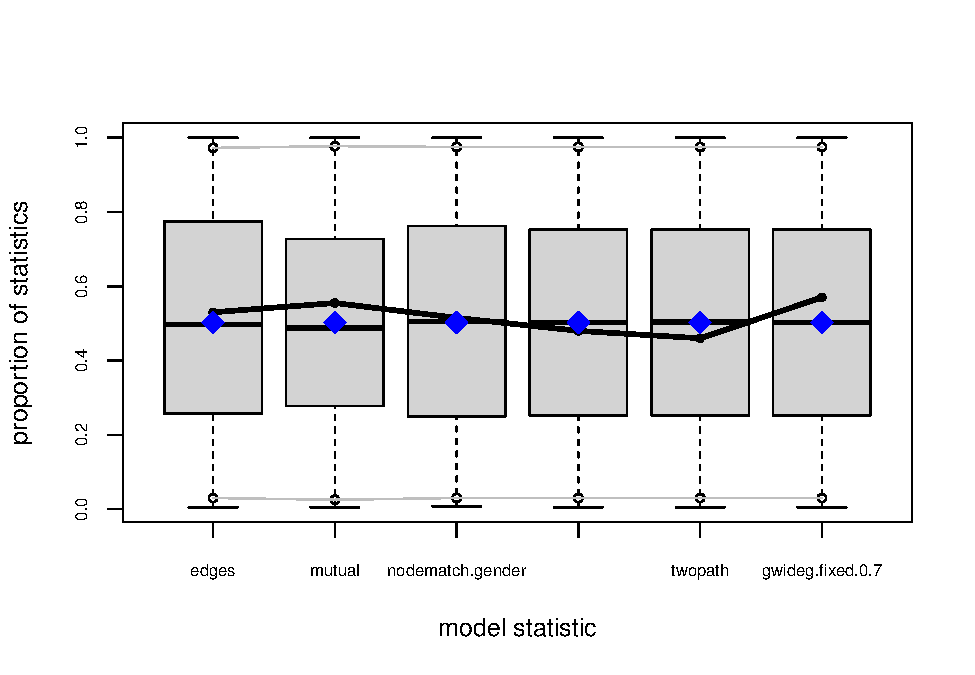
\includegraphics[keepaspectratio]{SNA-lab3.3_files/figure-pdf/fig-gof-friend-1.pdf}}

}

\end{minipage}%
%
\begin{minipage}{0.50\linewidth}

\subcaption{\label{fig-gof-friend-2}Outdegree distribution.}

\centering{

\pandocbounded{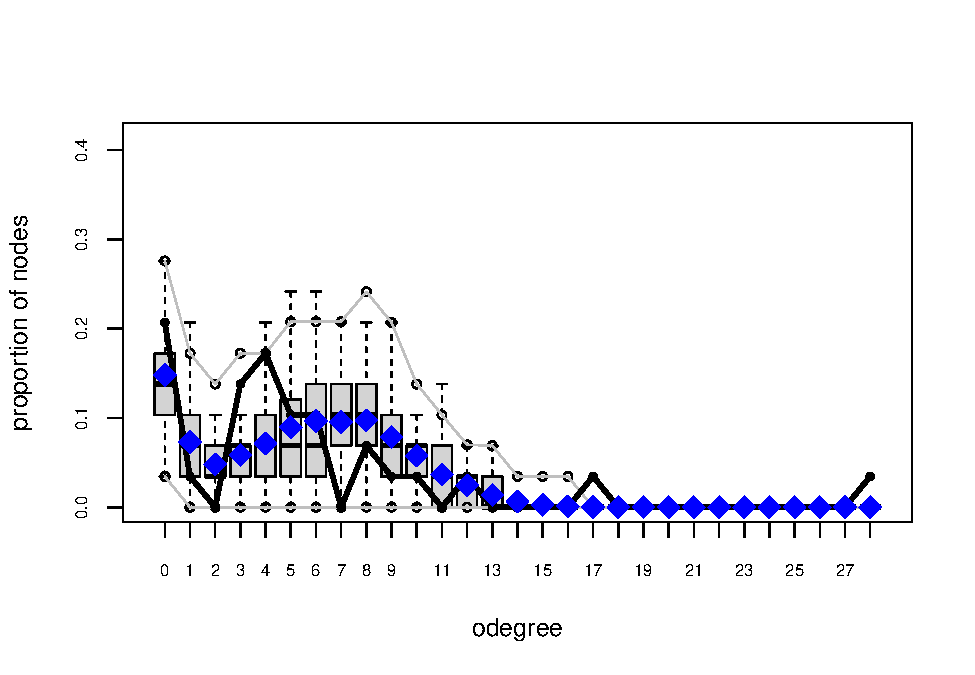
\includegraphics[keepaspectratio]{SNA-lab3.3_files/figure-pdf/fig-gof-friend-2.pdf}}

}

\end{minipage}%
\newline
\begin{minipage}{0.50\linewidth}

\subcaption{\label{fig-gof-friend-3}Indegree distribution.}

\centering{

\pandocbounded{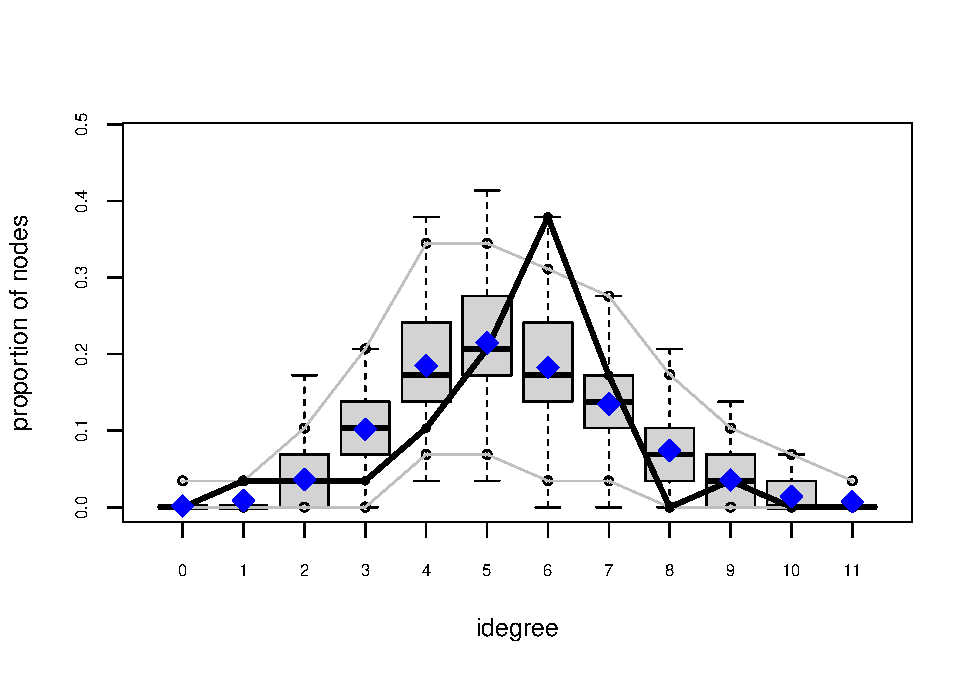
\includegraphics[keepaspectratio]{SNA-lab3.3_files/figure-pdf/fig-gof-friend-3.pdf}}

}

\end{minipage}%
%
\begin{minipage}{0.50\linewidth}

\subcaption{\label{fig-gof-friend-4}Edgewise shared partners.}

\centering{

\pandocbounded{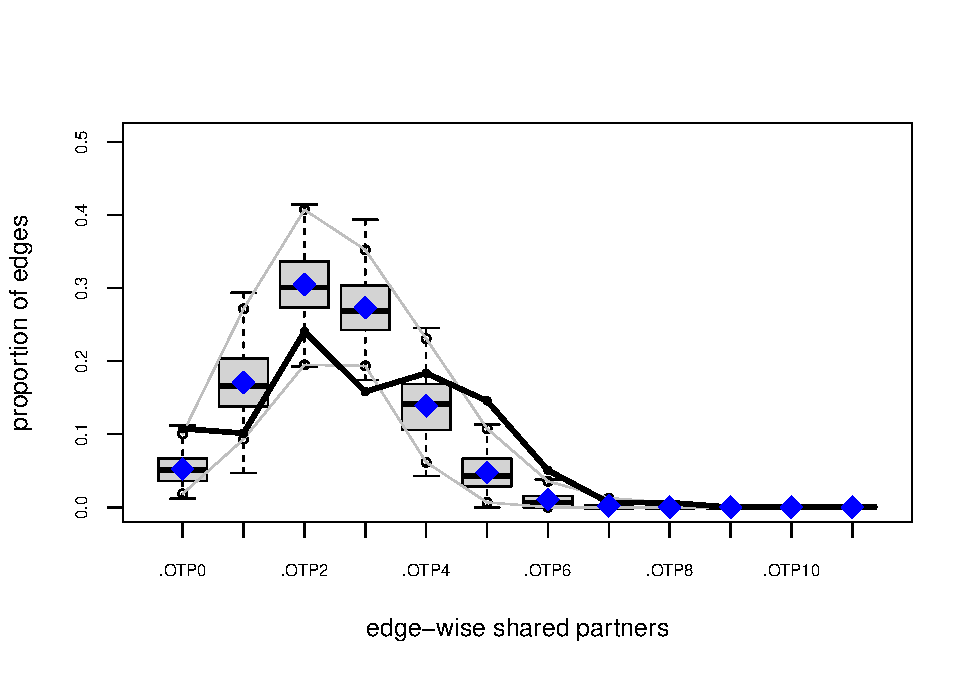
\includegraphics[keepaspectratio]{SNA-lab3.3_files/figure-pdf/fig-gof-friend-4.pdf}}

}

\end{minipage}%
\newline
\begin{minipage}{0.50\linewidth}

\subcaption{\label{fig-gof-friend-5}Minimum geodesic distance (including
unreachable dyads).}

\centering{

\pandocbounded{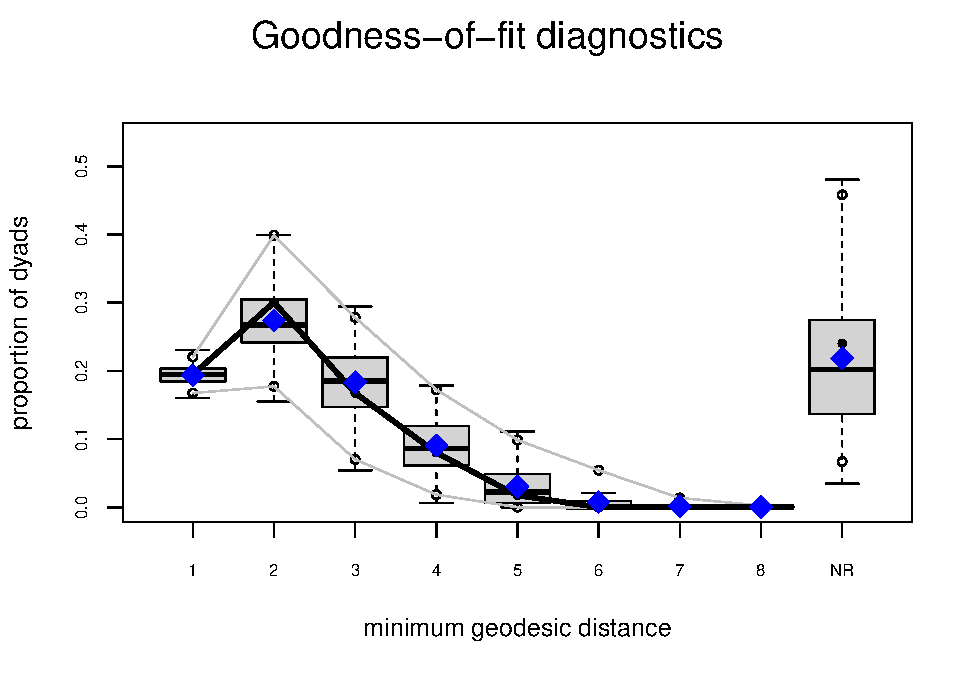
\includegraphics[keepaspectratio]{SNA-lab3.3_files/figure-pdf/fig-gof-friend-5.pdf}}

}

\end{minipage}%

\end{figure}%

\begin{figure}

\caption{\label{fig-gof-like}Goodness-of-fit diagnostics for the liking
ERGM.}

\begin{minipage}{0.50\linewidth}

\subcaption{\label{fig-gof-like-1}In-model terms.}

\centering{

\pandocbounded{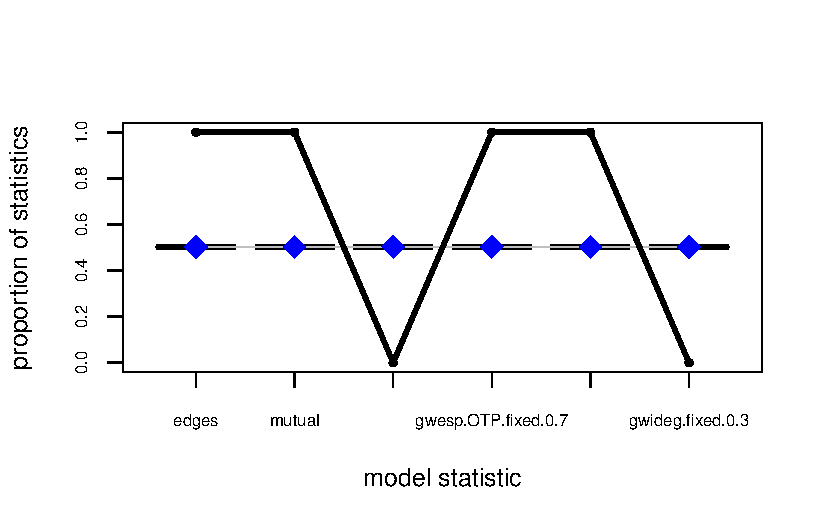
\includegraphics[keepaspectratio]{SNA-lab3.3_files/figure-pdf/fig-gof-like-1.pdf}}

}

\end{minipage}%
%
\begin{minipage}{0.50\linewidth}

\subcaption{\label{fig-gof-like-2}Outdegree distribution.}

\centering{

\pandocbounded{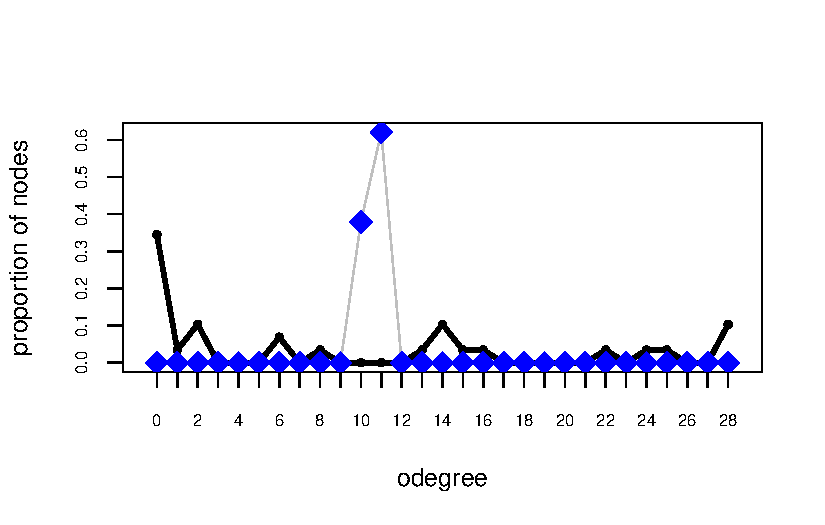
\includegraphics[keepaspectratio]{SNA-lab3.3_files/figure-pdf/fig-gof-like-2.pdf}}

}

\end{minipage}%
\newline
\begin{minipage}{0.50\linewidth}

\subcaption{\label{fig-gof-like-3}Indegree distribution.}

\centering{

\pandocbounded{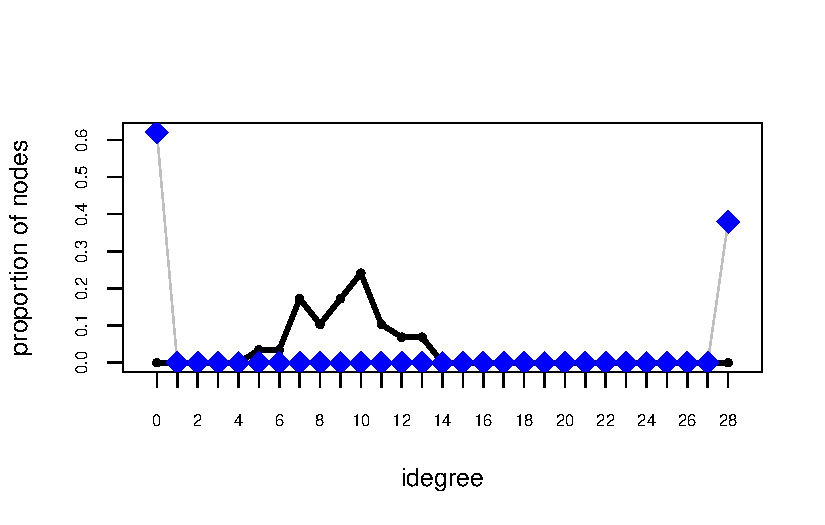
\includegraphics[keepaspectratio]{SNA-lab3.3_files/figure-pdf/fig-gof-like-3.pdf}}

}

\end{minipage}%
%
\begin{minipage}{0.50\linewidth}

\subcaption{\label{fig-gof-like-4}Edgewise shared partners.}

\centering{

\pandocbounded{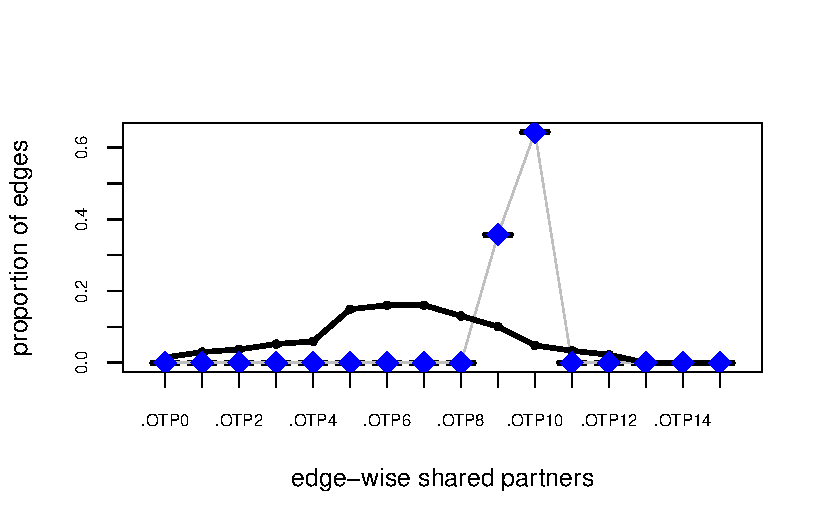
\includegraphics[keepaspectratio]{SNA-lab3.3_files/figure-pdf/fig-gof-like-4.pdf}}

}

\end{minipage}%
\newline
\begin{minipage}{0.50\linewidth}

\subcaption{\label{fig-gof-like-5}Minimum geodesic distance.}

\centering{

\pandocbounded{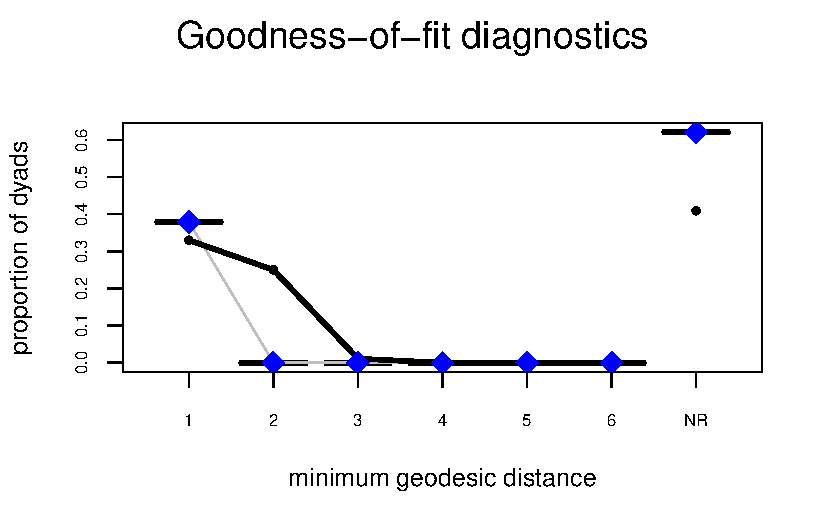
\includegraphics[keepaspectratio]{SNA-lab3.3_files/figure-pdf/fig-gof-like-5.pdf}}

}

\end{minipage}%

\end{figure}%

\begin{figure}

\caption{\label{fig-gof-popularity}Goodness of fit diagnostics for the
popularity ERGM.}

\begin{minipage}{0.50\linewidth}

\subcaption{\label{fig-gof-popularity-1}In model terms.}

\centering{

\pandocbounded{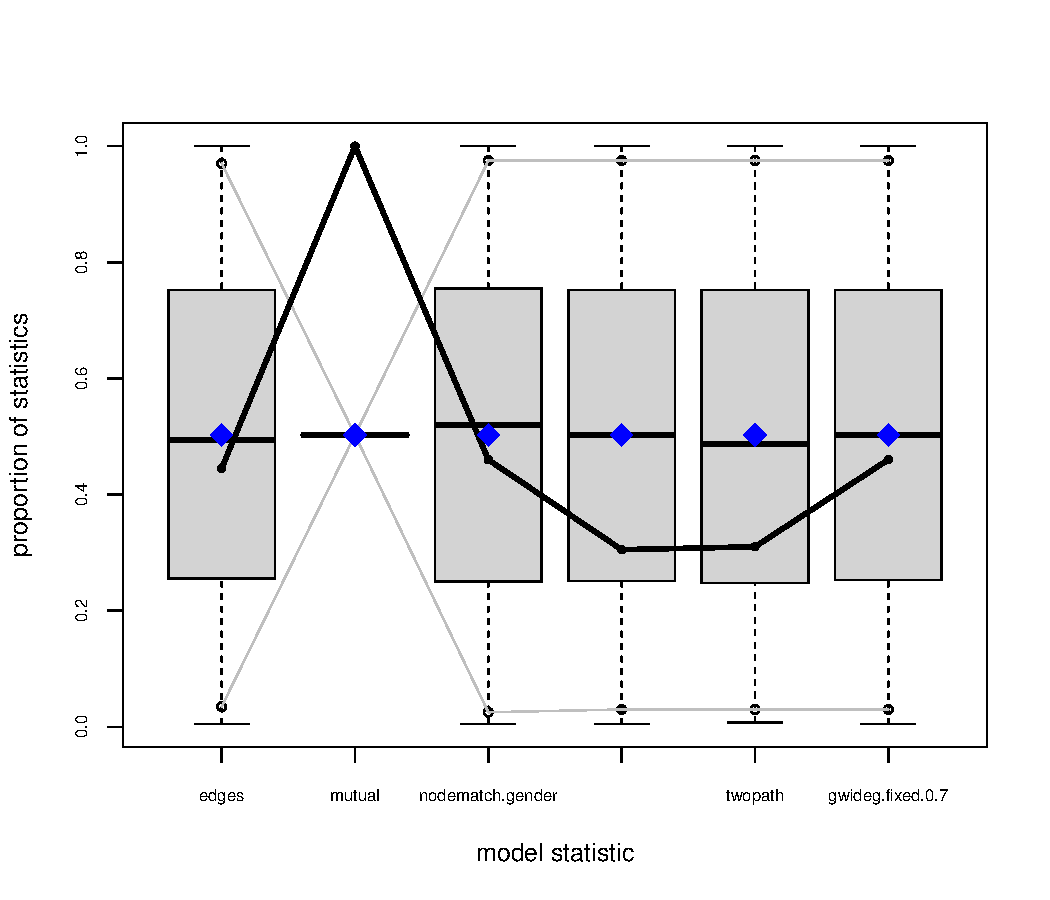
\includegraphics[keepaspectratio]{SNA-lab3.3_files/figure-pdf/fig-gof-popularity-1.pdf}}

}

\end{minipage}%
%
\begin{minipage}{0.50\linewidth}

\subcaption{\label{fig-gof-popularity-2}Outdegree distribution.}

\centering{

\pandocbounded{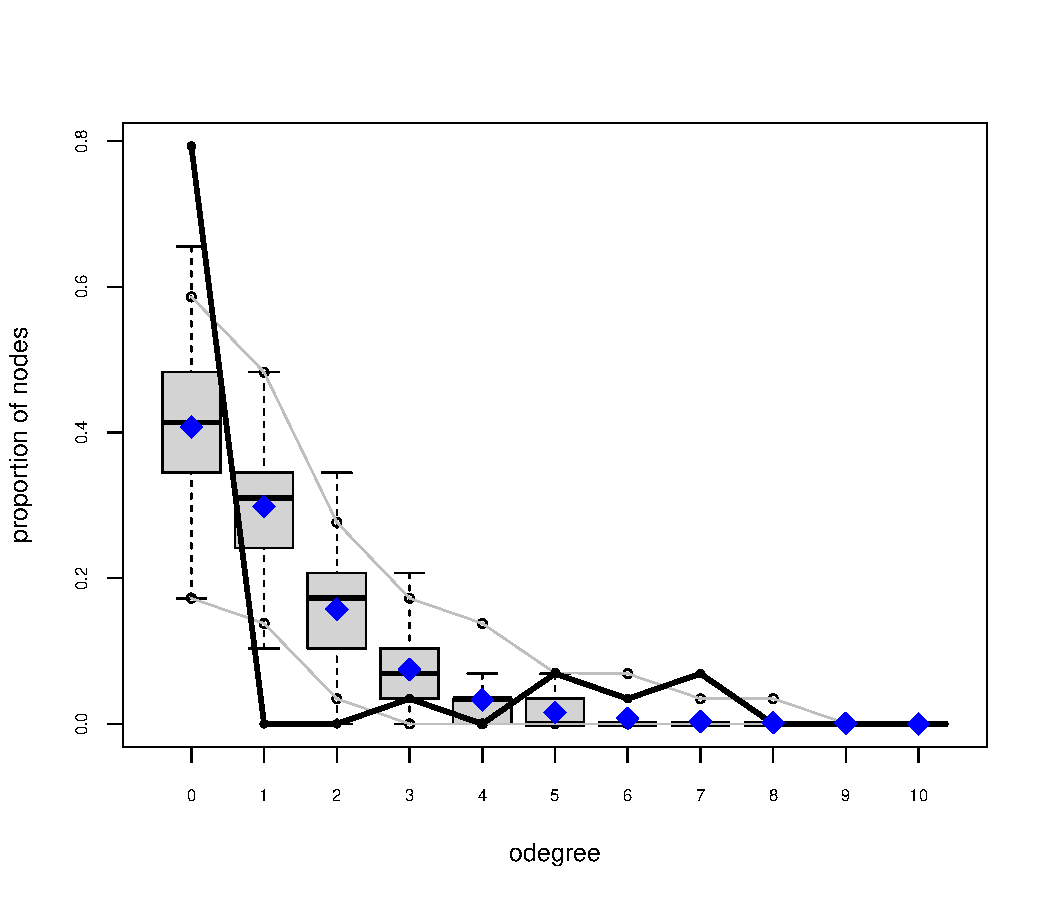
\includegraphics[keepaspectratio]{SNA-lab3.3_files/figure-pdf/fig-gof-popularity-2.pdf}}

}

\end{minipage}%
\newline
\begin{minipage}{0.50\linewidth}

\subcaption{\label{fig-gof-popularity-3}Indegree distribution.}

\centering{

\pandocbounded{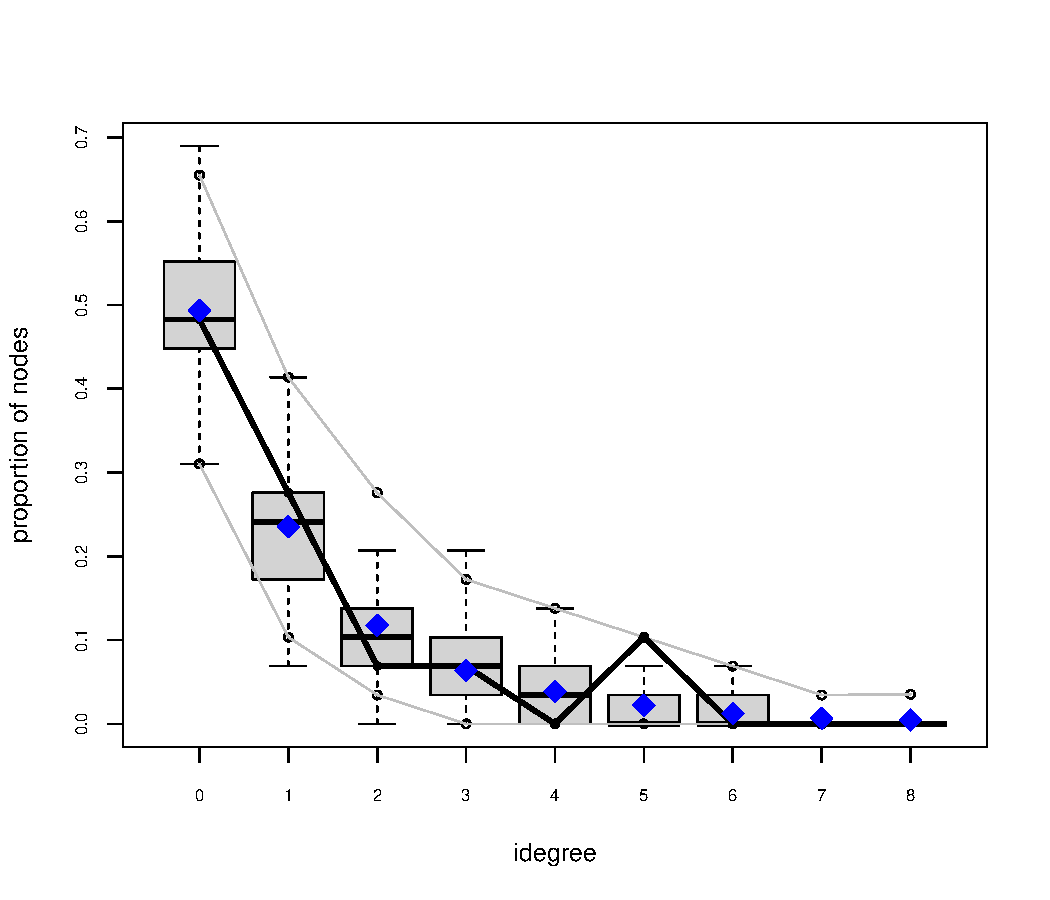
\includegraphics[keepaspectratio]{SNA-lab3.3_files/figure-pdf/fig-gof-popularity-3.pdf}}

}

\end{minipage}%
%
\begin{minipage}{0.50\linewidth}

\subcaption{\label{fig-gof-popularity-4}Edgewise shared partners.}

\centering{

\pandocbounded{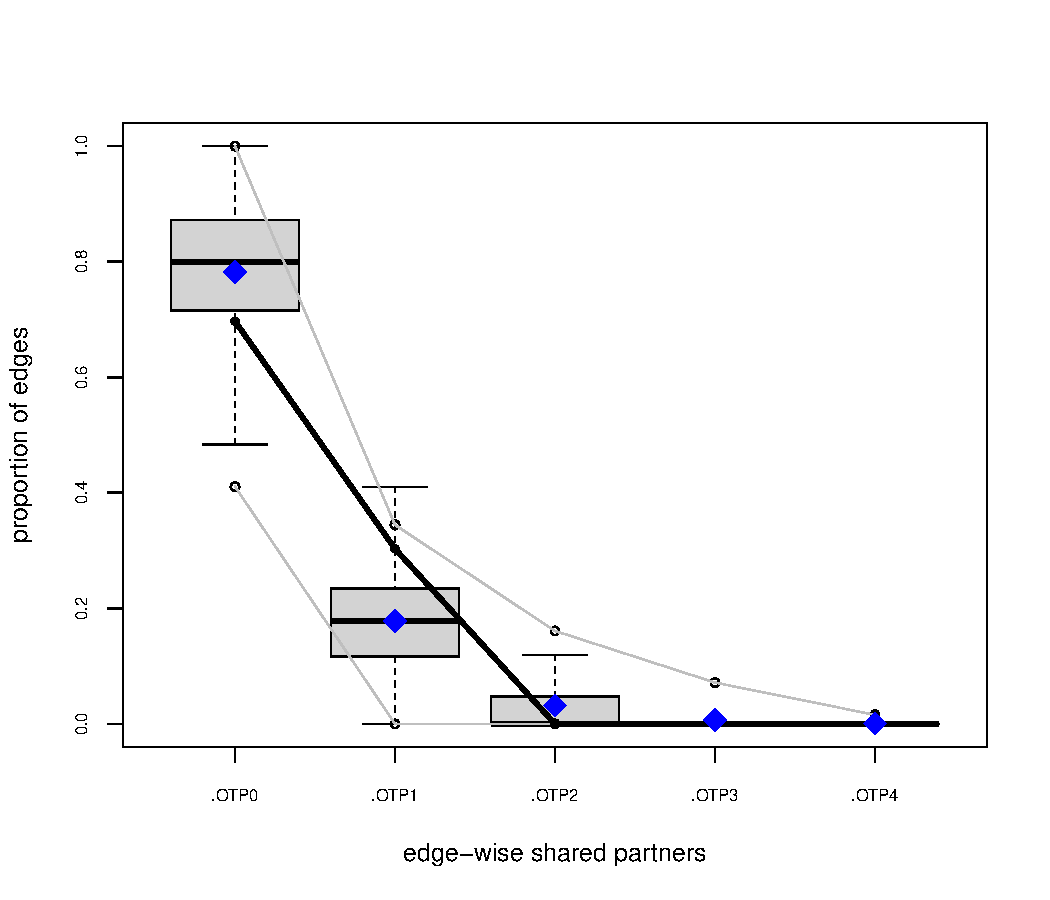
\includegraphics[keepaspectratio]{SNA-lab3.3_files/figure-pdf/fig-gof-popularity-4.pdf}}

}

\end{minipage}%
\newline
\begin{minipage}{0.50\linewidth}

\subcaption{\label{fig-gof-popularity-5}Minimum geodesic distance
(including unreachable dyads).}

\centering{

\pandocbounded{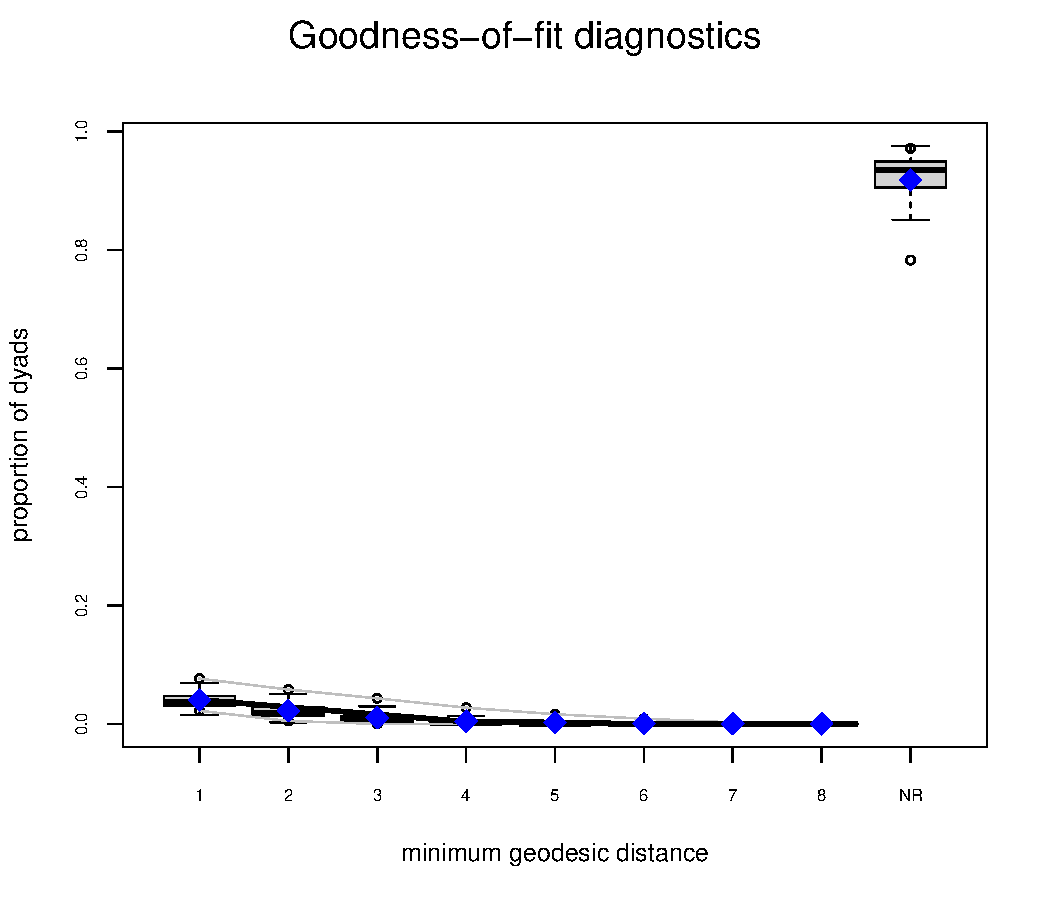
\includegraphics[keepaspectratio]{SNA-lab3.3_files/figure-pdf/fig-gof-popularity-5.pdf}}

}

\end{minipage}%

\end{figure}%

\begin{quote}
We assessed goodness of fit using standard ERGM GOF diagnostics,
comparing observed network statistics to distributions from networks
simulated from each fitted model, focusing on degree distributions,
edgewise shared partners, and minimum geodesic distance. The friendship
model provides the most satisfactory fit. In Fig. 1, the model
reproduces global connectivity reasonably well, and the geodesic
distance distribution is broadly consistent with the observed network.
The main mismatches are localized in the degree and shared-partner
diagnostics, where the observed indegree distribution is more sharply
peaked than the simulations, and the observed edgewise shared partner
proportions differ modestly around intermediate shared-partner counts.
Substantively, this means the fitted friendship ERGM captures core
clustering and reachability patterns, but it smooths some of the
observed heterogeneity in who nominates whom, and in how tightly
clustered ties are around common partners. The liking model shows poor
fit, consistent with the earlier instability. Fig 2 indicates that
simulated networks collapse to extreme and highly unrealistic degree and
shared-partner patterns, which fail to reproduce the observed
distributions. In plain terms, the fitted liking model under this
specification does not generate networks that look like the data, so
coefficients should not be treated as substantively meaningful. The
popularity model fits some aspects of the data but is mixed overall. Fig
3 shows that indegree, shared-partner, and distance patterns are
reproduced reasonably well for a very sparse nomination network, but the
outdegree distribution is notably misfit, with the observed mass at
outdegree zero exceeding the simulated envelope. Substantively, the
model captures the sparse, largely unreachable structure of the
popularity network, but it does not all capture heterogeneity in
nomination activity, meaning how many popularity nominations students
send. Together, the friendship model is the most stable and
substantively interpretable of the three under the imposed
specification, with popularity second and liking not adequate for
substantive inference \textgreater{}
\end{quote}

\subsection{10. Extended friendship ERGM with edgecov
effects}\label{extended-friendship-ergm-with-edgecov-effects}

\begin{longtable}[]{@{}ll@{}}

\caption{\label{tbl-q10-friendship-edgecov}Friendship ERGM with edgecov
effects of liking (acceptance) and popularity nominations. Entries show
estimate (SE).}

\tabularnewline

\toprule\noalign{}
Term & Estimate (SE) \\
\midrule\noalign{}
\endhead
\bottomrule\noalign{}
\endlastfoot
Edges & -3.688 (0.323) \\
Mutual & 0.491 (0.312) \\
Gender homophily (nodematch) & 0.266 (0.087) \\
Transitive closure (GWESP 0.7) & 1.632 (0.130) \\
Two-path & -0.175 (0.029) \\
Preferential attachment (GW indegree 0.7) & 2.987 (1.596) \\
Edgecov: liking nominations & 0.517 (0.147) \\
Edgecov: popularity nominations & 0.716 (0.368) \\

\end{longtable}

\subsection{11. Comparison with the simpler friendship
ERGM}\label{comparison-with-the-simpler-friendship-ergm}

\begin{quote}
In Exercise 10, we extended the friendship ERGM by adding the main
effects of liking and popularity nominations on friendship via
edgecov(). Comparing the extended friendship model (
Table~\ref{tbl-q10-friendship-edgecov}) to the simpler friendship model
from Exercise 6 (Table~\ref{tbl-ergm-comparison}), the core endogenous
mechanisms remain very similar. The edges term stays strongly negative,
indicating that the friendship network is sparse overall. Transitive
closure remains clearly positive, GWESP is 1.632 (SE 0.130) in the
extended model versus 1.738 (SE 0.131) in the simpler model, and the two
path term remains negative, −0.175 (SE 0.029) versus −0.169 (SE 0.031),
consistent with its stabilizing role. Gender homophily also remains
positive and of similar magnitude, 0.266 (SE 0.087) versus 0.314 (SE
0.074). Preferential attachment through GW indegree is still positive,
2.987 (SE 1.596) versus 3.271 (SE 1.556), suggesting that some
concentration of incoming friendship nominations persists even after
controlling for liking and popularity ties.
\end{quote}

\begin{quote}
The new exogenous covariate effects are both positive. Liking
nominations show a clear positive association with friendship ties,
0.517 (SE 0.147), implying that if student i likes student j, the
probability of an i→j friendship nomination is higher, net of
reciprocity, gender homophily, closure, and preferential attachment.
Popularity nominations are also positively related to friendship, 0.716
(SE 0.368), although the estimate is less precise. Substantively, this
pattern matches the idea that friendship is shaped by both relational
affect, captured by liking, and a reputational component, captured by
popularity.
\end{quote}

\begin{quote}
This comparison does bolster our reasoning in Exercise 2. We argued that
friendship combines status related visibility with relational
constraints, sitting between liking and popularity. In the extended
model, the friendship network still shows strong relational structure,
especially transitive closure, and also shows that both liking and
popularity ties independently predict friendship formation. This shows
that the view that friendship reflects a mixture of both processes of
liking and popularity, with strong local embedding through closure.
\end{quote}

\subsection{12. Collaboration statement}\label{collaboration-statement}

\begin{quote}
This assignment was completed in collaboration of Patricia and Ahsan. We
discussed the theoretical expectations, model specification, and
interpretation of the ERGM results together. In particular, discussions
about model convergence issues and the interpretation of the
preferential attachment term were especially helpful for clarifying the
comparison across networks. Writing and interpretation presented here
reflect our understanding of the tasks.
\end{quote}




\end{document}
